% You can write any comments you want as long as there is a percentage sign at the beginning. This won't appear in your document.

\documentclass[12pt]{article}
%	options include 12pt or 11pt or 10pt
%	classes include article, report, book, letter, thesis, with 'article' being the default layout

\usepackage{amssymb,amsmath,textcomp} %These are optional packages you can install which gives you more mathematical symbols to play with

\usepackage{graphicx} %This allows you to insert jpg, png and pdf files into the document
\graphicspath{{img/}}
\usepackage{enumerate}


\title{Introduction to Vision and Robotics\\Vision Practical: Coin Counter}
\author{Dylan Angus, Matthew Martin}
\date{\today}

%%%%%%%%%%%%%%%%%%%%%%%%%%%%%%%%%%%%

% OUTLINE
% Introduction
%	a paragraph outlining the task and main ideas we used to solve it
% Methods
%	for each technique we used for background subtraction
%		list their advantages and disadvantages
%		provide images of their output
%		explain why we decided to/not to use it
%	for each technique of object segmentation/separation
%		list their advantages and disadvantages
%		provide images of their output
%		explain why we decided to/not to use it
%	explain our classifier
% Results
%	provide data (e.g. confusion matrix) for how our classifier performed under testing
%	show output images from each stage of our program
% Discussion
%	discuss the success of our program, how it could be improved, challenges/limitations we faced
% Code
%	attach all matlab code that we wrote (not anything downloaded from course website)as an appendix

%%%%%%%%%%%%%%%%%%%%%%%%%%%%%%%%%%%%%

\begin{document}
	
\maketitle

\section{Introduction}

The purpose of this practical is to develop a program in Matlab that recognises and classifies several objects in an image. These objects can be coins or other small items, and the program must segment the image, identify each of the objects, and output the total value (in pounds and pence) of the objects in the image.

All of the images are taken from a downward facing camera viewing a scene containing the objects on a static background. We were provided with a set of 14 sample images on which to train our classifier (see Figure \ref{samplescene} for an example).

\begin{figure}
	\centering
	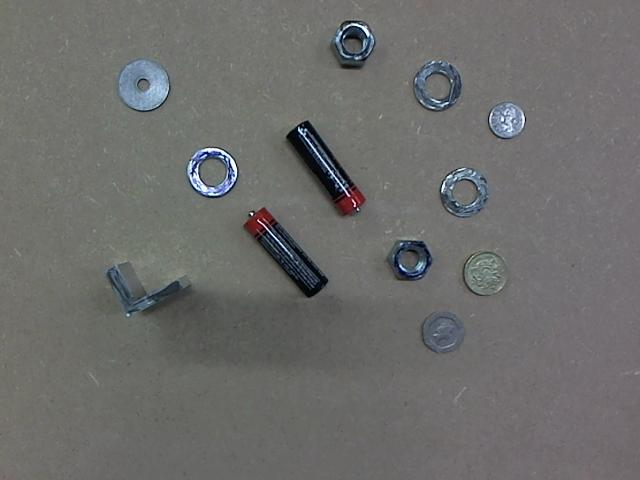
\includegraphics[width=0.75\linewidth]{02}
	\label{samplescene}
	\caption{This is one of the test images given to train the classifier.}
\end{figure}

The following are the objects and associated values that may or may not be present in any given image:
\begin{itemize}
	\item one and two pound pieces
	\item 50, 20, and 5 pence pieces
	\item washer with small hole (75p)
	\item washer with large hole (25p)
	\item angle bracket (2p)
	\item AAA battery (no value)
	\item nut (no value)
\end{itemize}

We approached this problem by dividing it into three distinct stages: background segmentation, object detection, and object classification.

\section{Methods}

\subsection{Background Segmentation}

\subsection{Object Detection}

\subsection{Classification}

\section{Results}

\section{Discussion}

\section*{Appendix}

\begin{verbatim}
	
	code can go inside these tags 
	\begin{verbatim} 
	.... 
	\ end{verbatim} (no space though)
	
\end{verbatim}


\end{document}